\documentclass[utf8]{beamer}
\usetheme{Dresden}
\usepackage[T1]{fontenc}
\usepackage{tikz}
\usepackage{caption}
\usepackage{subfigure}


%dodatak za programski kod
\usepackage{listings}
\usepackage{color}
\usepackage{setspace}
\definecolor{dkgreen}{rgb}{0,0.6,0}
\definecolor{gray}{rgb}{0.5,0.5,0.5}
\definecolor{mauve}{rgb}{0.58,0,0.82}

\lstset{frame=tb,
  language=Java,
  aboveskip=3mm,
  belowskip=3mm,
  showstringspaces=false,
  columns=flexible,
  basicstyle={\small\ttfamily},
  numbers=left,
  numberstyle=\small\color{gray},
  keywordstyle=\color{blue},
  commentstyle=\color{dkgreen},
  stringstyle=\color{mauve},
  breaklines=true,
  breakatwhitespace=true,
  tabsize=2
}

\renewcommand{\figurename}{Slika}
% Postavljanje fonta
\if@fonttimes\RequirePackage{times} \fi
\if@fontlmodern\RequirePackage{lmodern} \fi

\usecolortheme{dolphin}

%prikaz broja slajda
\expandafter\def\expandafter\insertshorttitle\expandafter{%
	\insertshorttitle\hfill%
	\insertframenumber\,/\,\inserttotalframenumber}

\newcommand{\engl}[1]{(engl.~\emph{#1})}
\newcommand{\putat}[3]{\begin{picture}(0,0)(0,0)\put(#1,#2){#3}\end{picture}}

\title[Neighbour joining]{Neighbour joining}

\author[Dino Šantl]{Bioinformatika - projekt \newline\newline 
				 \itshape		{Filip Beć}\\
				 \itshape{Zorana Ćurković}\\
				 \itshape{Goran Gašić}\\
				 \itshape{Melita Kokot}\\
				 \itshape{Dino Šantl}\\
				 \itshape{Igor Smolkovič}
}

\institute{Fakultet elektrotehnike i računarstva}
\date{Zagreb, siječanj 2014.}
\begin{document}

\begin{frame}
\titlepage
\end{frame}

\section{Uvod}
\begin{frame}{Uvod}
\begin{itemize}
	\item Izgradnja filogenetskog stabla
	\item Od dna prema vrhu
	\item Pohlepan algoritam - minimizira udaljenosti u svakom koraku
	\item Vremenska složenost $O(N^3)$
	\item Memorijska složenost $O(N^2)$
\end{itemize}
\end{frame}

\section{Opis algoritma}
\begin{frame}{Opis algoritma}
\begin{enumerate}
	\item Ulaz je matrica udaljenosti između genoma 
	\pause
	\item Iz matrice udaljenosti računa se nova matrica - Q
	\pause
	\item U matrici Q pronalazi se minimalna vrijednost između dva čvora
	\pause
	\item Pronađena dva čvora spajaju se s novim čvorom
	\pause
	\item Iz matrice udaljenosti brišu se dva odabrana čvora i dodaje se
novi čvor
	\pause
	\item Ako matrica udaljenosti sadrži više od tri čvora, skoči na 2. korak
	\pause
	\item Završni korak spajanja zadnja tri čvora s novim čvorom
\end{enumerate}
\end{frame}

\begin{frame}{Opis algoritma}
\begin{figure}[htb]
\centering
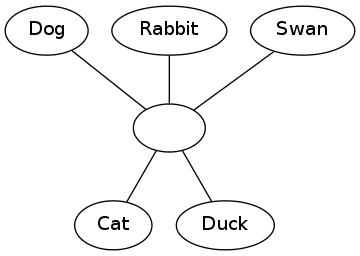
\includegraphics[scale=0.5]{../Dokumentacija/img/pocetni.png}
\caption{Početno stablo}
\end{figure}
\end{frame}

\begin{frame}{Opis algoritma}
\begin{figure}[htb]
\centering
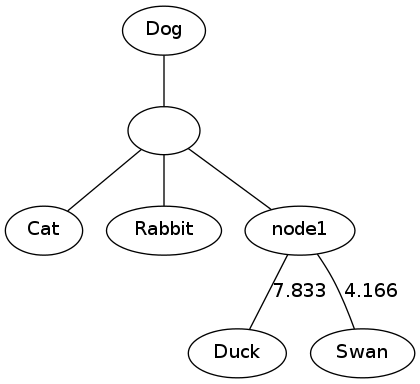
\includegraphics[scale=0.4]{../Dokumentacija/img/prvi.png}
\caption{Prvi korak}
\end{figure}
\end{frame}

\begin{frame}{Opis algoritma}
\begin{figure}[htb]
\centering
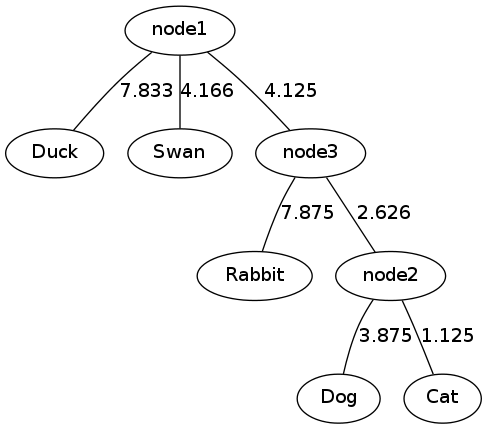
\includegraphics[scale=0.4]{../Dokumentacija/img/zadnji.png}
\caption{Zadnji korak}
\end{figure}
\end{frame}

\begin{frame}{Opis algoritma - VAŽNO!}
\begin{itemize}
\item Računanje matrice Q i to $N-3$ puta kao: 
$$ Q(i,j) = (N-2) d(i,j) - \sum_{k=1}^{N}d(i,k) - \sum_{k=1}^{N}d(j,k) $$
\item Direktna implementacija: $O(N^4)$
\item Sume računati prije
\end{itemize}
\end{frame}


\section{Rezultati}
\begin{frame}{Rezultati}
\begin{itemize}
	\item Izgrađena infrastruktura
	\item Računanje udaljenosti iz FASTA datoteke i povezivanje s implementacijama
	\item Lakše testiranje - izlaz je vizualni prikaz stabla
	\item Točnost - skripta koja uspoređuje dva grafa
	\item NJ nije deterministički!
\end{itemize}
\end{frame}

\begin{frame}{Rezultati}
\begin{itemize}
	\item Filip Beć - \textbf{Objective-C}
	\item Zorana Ćurković - \textbf{Python}
	\item Goran Gašić - \textbf{Java}
	\item Melita Kokot - \textbf{Ruby}
	\item Dino Šantl - \textbf{C}
	\item Igor Smolkovič - \textbf{C++}
\end{itemize}
\end{frame}

\begin{frame}{Vrijeme}
\begin{figure}
\centering
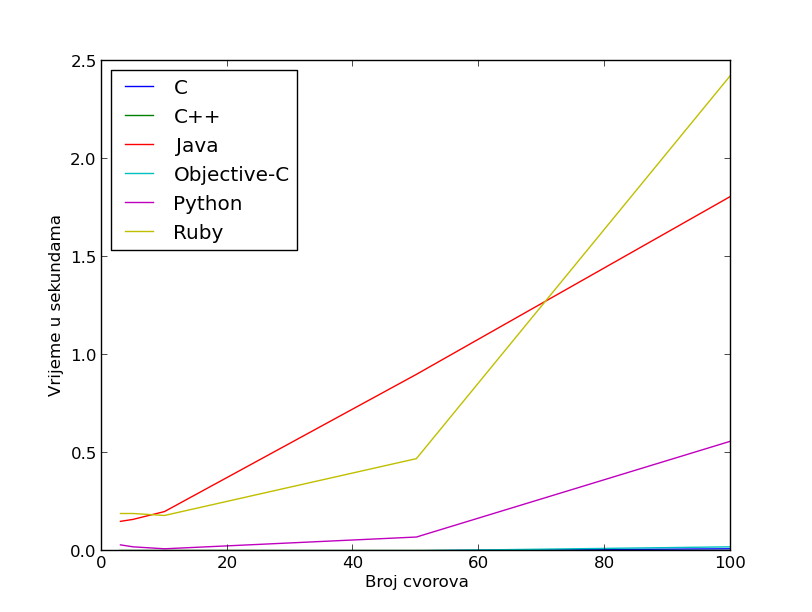
\includegraphics[scale=0.45]{../Dokumentacija/img/Primjeri_do_100.png}
\end{figure}
\end{frame}

\begin{frame}{Vrijeme}
\begin{figure}
\centering
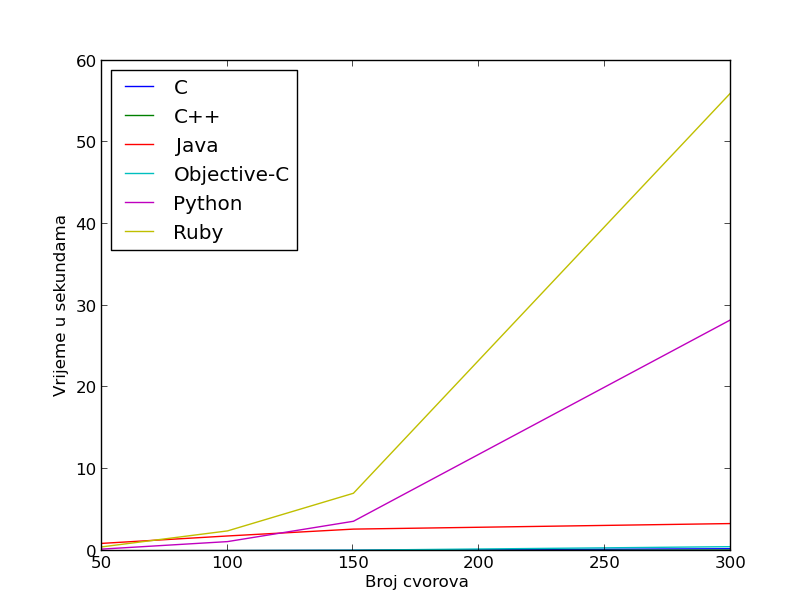
\includegraphics[scale=0.45]{../Dokumentacija/img/Primjeri_50_300.png}
\caption{Vremena izvođenja algoritama za veličine od 50 to 300 čvorova}
\label{fig:time_50_300}
\end{figure}
\end{frame}

\begin{frame}{Vrijeme}
\begin{figure}
\centering
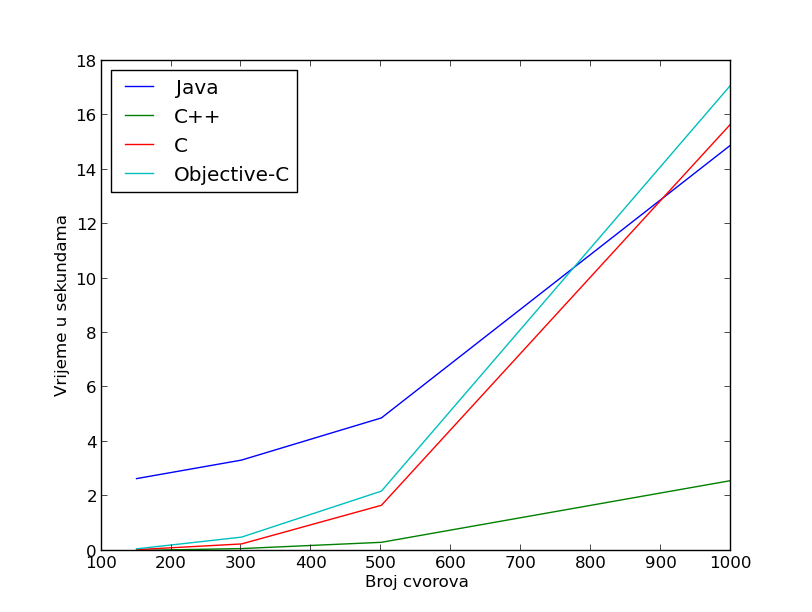
\includegraphics[scale=0.45]{../Dokumentacija/img/Primjeri_150_1000.png}
\caption{Vremena izvođenja za primjere od 150 do 1000 čvorova}
\label{fig:time_150_1000}
\end{figure}
\end{frame}

\begin{frame}{Memorija}

\begin{figure}
\centering
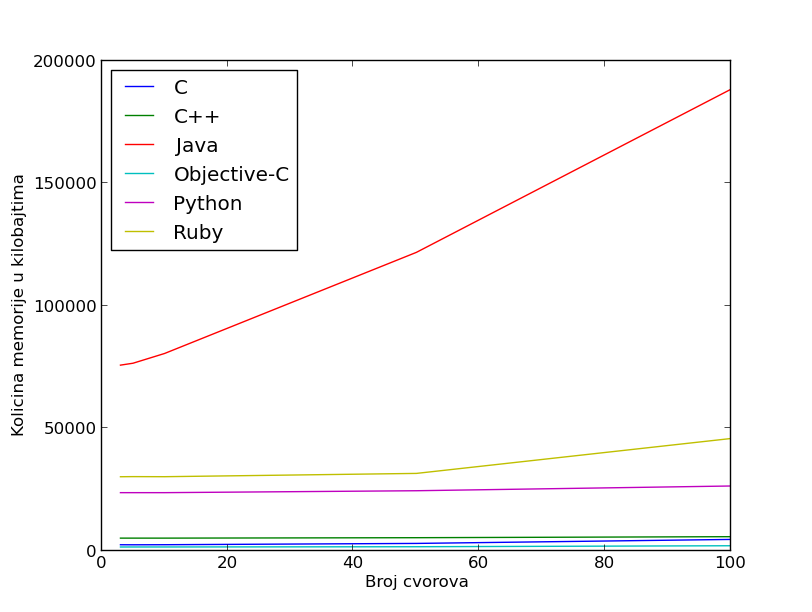
\includegraphics[scale=0.45]{../Dokumentacija/img/memorija_100.png}
\caption{Korištena memorija u kilobajtima do 100 čvorova}
\label{fig:memorija_100}
\end{figure}

\end{frame}

\begin{frame}{Memorija}

\begin{figure}[!h]
\centering
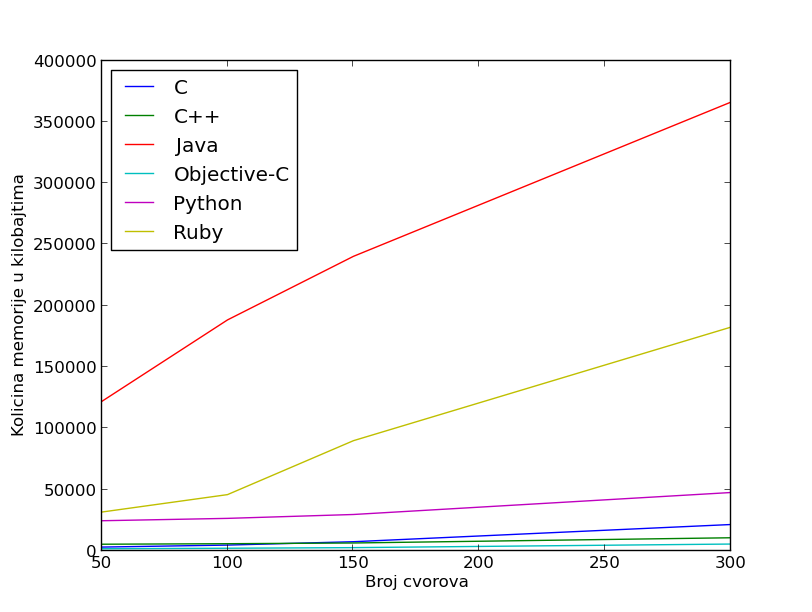
\includegraphics[scale=0.45]{../Dokumentacija/img/memorija_300.png}
\caption{Korištena memorija u kilobajtima od 50 do 300 čvorova}
\label{fig:memorija_300}
\end{figure}

\end{frame}

\begin{frame}{Memorija}

\begin{figure}[!h]
\centering
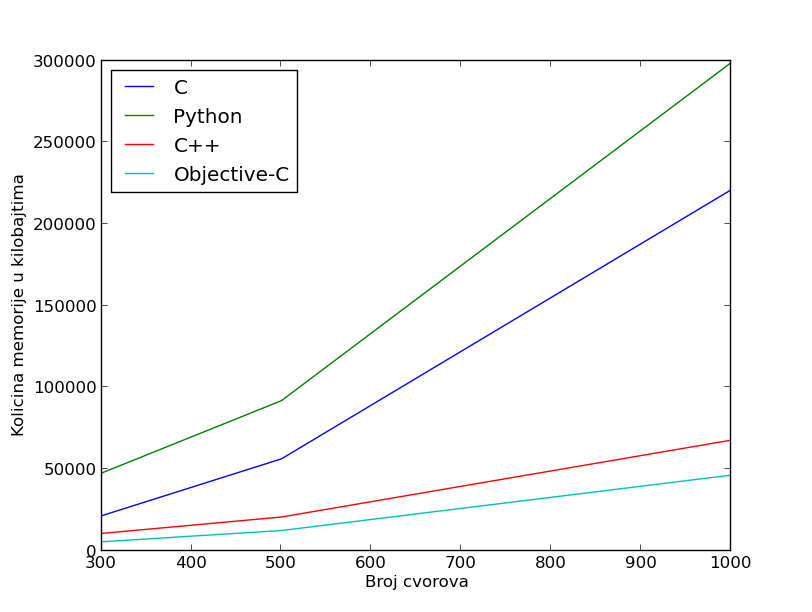
\includegraphics[scale=0.45]{../Dokumentacija/img/memorija_1000.png}
\caption{Korištena memorija od 300 do 1000 čvorova}
\label{fig:memorija_1000}
\end{figure}
\end{frame}


\section*{}
\begin{frame}{}
\huge{Hvala na pažnji!}
\end{frame}

\end{document}